\begin{transitionframe}
\textbf{Part E:}

Criticisms
\end{transitionframe}

\begin{frame}{Criticisms}{S5}

\end{frame}


\begin{frame}{Criticisms}{Modal Collapse}

\end{frame}


\begin{frame}{Criticisms}{No Neutral Properties}

\end{frame}



\begin{transitionframe}
\textbf{Part F:}

Conclusions
\end{transitionframe}



\begin{frame}{Summary of Results about the Ontological Proof}
\begin{itemize}[<+->]
\item K sufficient for T1, C1 and T2 
\item S5 not needed for T3
\item KB sufficient for T3 
\item A simpler new proof of C1
\item G\"odel's original axioms (without conjunct $\phi(x)$ in D2) are inconsistent
\item Scott's axioms are consistent
\item For T1, only half of A1 (A1a) is needed 
\item For T2, the other half (A1b) is needed
\end{itemize}
\end{frame}


\begin{frame}{Summary of Results for Logic} \small
\begin{itemize}[<+->]
\item Infra-structure for reasoning with modal logic using existing proof assistants and higher-order automated theorem provers
\item A new natural deduction calculus for higher-order modal logic
\end{itemize}
\end{frame}

\begin{frame}[plain]
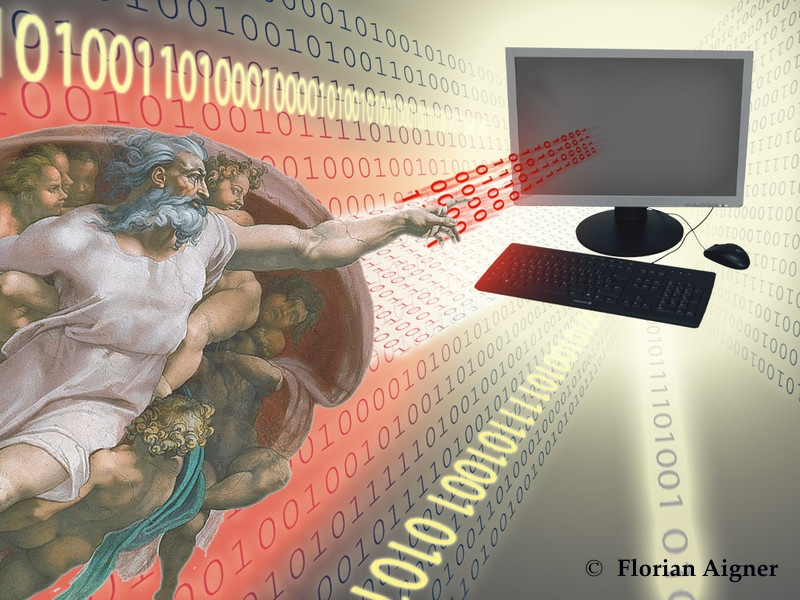
\includegraphics[width=\textwidth]{TUWien-GodComputerC} 
\end{frame}
